\section{Efficient Constrained Decoding with Compressed Finite State Machine}
\label{sec:compressed-fsm}

In LM programs, users often want to constrain the model's output to follow specific formats, such as JSON schemas. This can improve controllability and robustness, and make the output easier to parse. \lang offers a \texttt{regex} argument to enforce such constraints using regular expressions, which are expressive enough for many practical scenarios.
Existing systems support this by converting a regular expression into a finite state machine (FSM)~\cite{willard2023efficient}. During decoding, they maintain the current FSM state, retrieve allowed tokens from the next states, and set the probability of invalid tokens to zero, decoding token by token. This token-by-token approach, however, is inefficient when there are opportunities to decode multiple tokens at once.
For example, the constant sequence \texttt{\{"summary":\ "} in \autoref{fig:example_first_program} spans multiple tokens in the normal decoding process as shown in \autoref{fig:example_compressed_fsm} (c), requiring multiple decoding stages, even though there is only one valid next token when decoding it. Therefore, the whole sequence can be decoded in a single step (i.e., forward pass).
However, existing systems can only decode one token at a time because the lack of integration between the FSM and the model runner in existing systems prevents multi-token processing, resulting in slow decoding.


\begin{figure}[t]
\centering
\vspace{-2em}
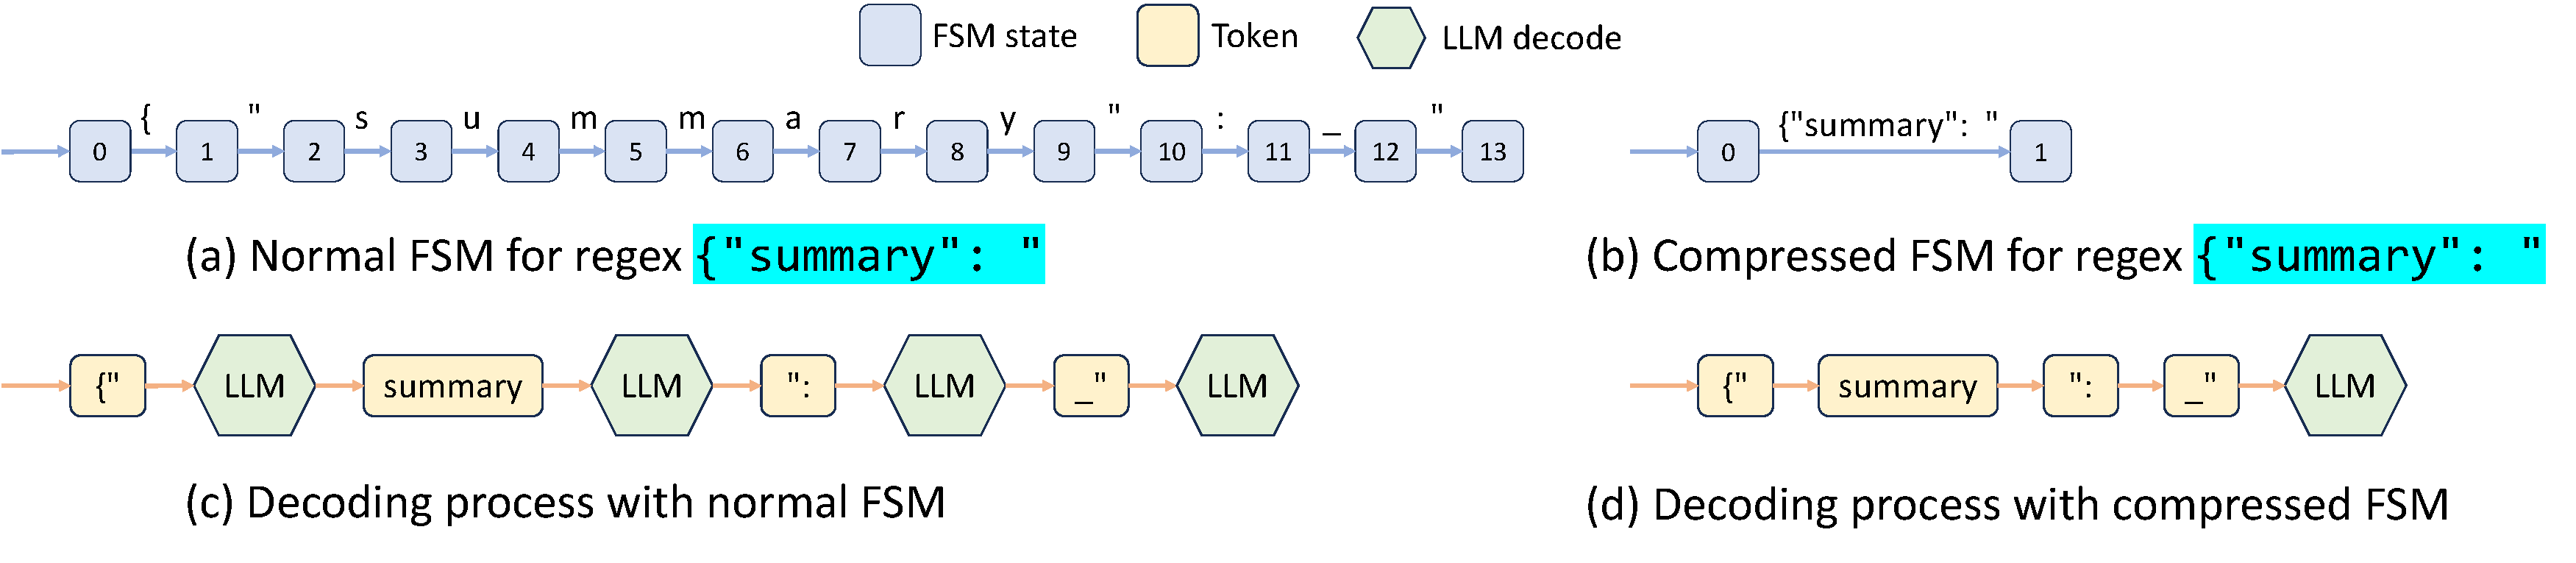
\includegraphics[width=0.99\linewidth]{figures/example_compressed_fsm.pdf}
\vspace{-0.5em}
\caption{The decoding process of normal and compressed FSMs (the underscore \texttt{\_} means a space).}
\vspace{-1.5em}
\label{fig:example_compressed_fsm}
\end{figure}

\lang overcomes this limitation by creating a fast constrained decoding runtime with a compressed FSM. This runtime analyzes the FSM and compresses adjacent singular-transition edges in the FSM into single edges as demonstrated in \autoref{fig:example_compressed_fsm} (b), allowing it to recognize when multiple tokens can be decoded together. In \autoref{fig:example_compressed_fsm} (d), multiple tokens on the compressed transition edge can be decoded in one forward pass, which greatly accelerates the decoding process. It is also general and applicable to all regular expressions. More details on the background and implementation are in \autoref{sec:additional_fsm}.









